\documentclass[11pt,a4paper,twoside]{article}

% LaTeX-Umsetzung der "Richtlinien für Projekt- und Diplomarbeiten"
% der LFE Medieninformatik, LMU München. (Autor: Richard Atterer, 27.9.2006, 23.10.2007), Bug-Fixing Mark Kaczkowski (23.6.2008)

\usepackage[T1]{fontenc} % sonst geht \hyphenation nicht mit Umlauten
%\usepackage[latin1]{inputenc} % man kann schreiben äöüß statt "a"o"u"s
\usepackage[utf8]{inputenc} % wie oben, aber UTF-8 als Encoding statt ISO-8859-1 (latin1)
\usepackage[ngerman,british]{babel} % deutsche Trennregeln, "Inhaltsverzeichnis" etc.
%\usepackage{ngerman} % Alternative zum Babel-Paket oben
\usepackage{mathptmx} % Times-Roman-Schrift (auch für mathematische Formeln)
\usepackage{listings}

% Zum Setzen von URLs
\usepackage{color}
\definecolor{darkred}{rgb}{.25,0,0}
\definecolor{darkgreen}{rgb}{0,.2,0}
\definecolor{darkmagenta}{rgb}{.2,0,.2}
\definecolor{darkcyan}{rgb}{0,.15,.15}
\usepackage[plainpages=false,bookmarks=true,bookmarksopen=true,colorlinks=true,
  linkcolor=darkred,citecolor=darkgreen,filecolor=darkmagenta,
  menucolor=darkred,urlcolor=darkcyan]{hyperref}

% pdflatex: Bilder in den Formaten .jpeg, .png und .pdf
% latex: Bilder im .eps-Format
\usepackage{graphicx}

\usepackage{fancyhdr} % Positionierung der Seitenzahlen
\fancyhead[LE,RO,LO,RE]{}
\fancyfoot[CE,CO,RE,LO]{}
\fancyfoot[LE,RO]{\Roman{page}}
\renewcommand{\headrulewidth}{0pt}
\setlength{\headheight}{13.6pt} % behebt headheight Warning

% Korrektes Format für Nummerierung von Abbildungen (figure) und
% Tabellen (table): <Kapitelnummer>.<Abbildungsnummer>
\makeatletter
\@addtoreset{figure}{section}
\renewcommand{\thefigure}{\thesection.\arabic{figure}}
\@addtoreset{table}{section}
\renewcommand{\thetable}{\thesection.\arabic{table}}
\makeatother

\sloppy % Damit LaTeX nicht so viel über "overfull hbox" u.ä. meckert

% Ränder
\addtolength{\topmargin}{-16mm}
\setlength{\oddsidemargin}{25mm}
\setlength{\evensidemargin}{35mm}
\addtolength{\oddsidemargin}{-1in}
\addtolength{\evensidemargin}{-1in}
\setlength{\textwidth}{15cm}
\addtolength{\textheight}{34mm}

% Listings formatieren
\lstset{basicstyle=\ttfamily\color{blue}}

%______________________________________________________________________

\begin{document}

\pagestyle{empty} % Vorerst keine Seitenzahlen
\pagenumbering{alph} % Unsichtbare alphabetische Nummerierung

\begin{center}
\textsc{Ludwig-Maximilians-Universität München}\\
Department ``Institut für Informatik''\\
Lehr- und Forschungseinheit Medieninformatik\\
Prof.\ Dr.\ Heinrich Hußmann

\vspace{5cm}
{\large\textbf{Bachelor's Thesis}}\vspace{.5cm}

{\LARGE Using Keyword Extraction for Image Retrieval in News Articles}\vspace{.3cm}

{\Large Comparison of Different Approaches}\vspace{1cm}

{\large Martin Schön}\\\href{mailto:martingeorg.schoen@gmail.com}{martingeorg.schoen@gmail.com}

\end{center}
\vfill

\begin{tabular}{ll}
Bearbeitungszeitraum: & 1. 6. 2018 bis 19. 10. 2018\\
%Externer Betreuer: & Manfred Manager\\
Verantw. Hochschullehrer: & Prof. Dr. Neil Thurman
\end{tabular}
%______________________________________________________________________

\clearpage
\selectlanguage{british}
\section*{Abstract}

Short abstract of the work, maximum of 250 words.

\selectlanguage{ngerman}
\clearpage
\section*{Aufgabenstellung}

Kopie der Original-Aufgabenstellung

\vfill % Sorgt dafür, dass das Folgende an das Seitenende rutscht

\noindent Ich erkläre hiermit, dass ich die vorliegende Arbeit
selbstständig angefertigt, alle Zitate als solche kenntlich gemacht
sowie alle benutzten Quellen und Hilfsmittel angegeben habe.

\bigskip\noindent Berlin, \today

\vspace{4ex}\noindent\makebox[7cm]{\dotfill}

%______________________________________________________________________

\selectlanguage{british}
\cleardoublepage
\pagestyle{fancy}
\pagenumbering{roman} % Römische Seitenzahlen
\setcounter{page}{1}

% Inhaltsverzeichnis erzeugen
\tableofcontents

%Abbildungsverzeichnis erzeugen - normalerweise nicht nötig
%\cleardoublepage
%\listoffigures
%______________________________________________________________________

\cleardoublepage

% Arabische Seitenzahlen
\pagenumbering{arabic}
\setcounter{page}{1}
% Geändertes Format für Seitenränder, arabische Seitenzahlen
\fancyhead[LE,RO]{\rightmark}
\fancyhead[LO,RE]{\leftmark}
\fancyfoot[LE,RO]{\thepage}

\section{Introduction}

Automated Journalism has gained significant momentum in recent years. Media outlets from all over the world are starting to use software systems based on artificial intelligence to augment or fully automate tasks that were once done by human editors. Whereas lots of research has been invested in automating tasks related to the writing of news articles, with some applications already being used in production\footnote{The best-known application is probably Automated Insight's Wordsmith application that artificially generates stories for customers like the Associated Press.\cite{AssociatedPressAutomatedInsights}}, fewer attention has been paid to the visual components of a written news story. 

This work aims to tackle one specific but very common issue in present-day newsrooms: Written news articles are usually illustrated with a photograph accompanying the story - especially in digital environments such as websites and mobile applications. This happens for a variety of reasons, some of which are outlined in section \ref{TheoryPerception}. Even though time consuming, this task can in many cases be repetitive and tedious for humans, since news stories do not always leave much room for creative image selection: In many cases, the best solution is depicting one of the key actors or central topics of an article.

Nevertheless, even though trivial for humans, this task is highly complex for a machine to solve: Figuring out key aspects of a story and selecting appropriate images (which might in many cases mean showing something closely related to the topic or even symbolising it) is a problem that is hard to define in mathematical terms. This thesis aims to contribute to the automation of this task by presenting a system that makes use of certain features inherent to the domain of written news articles, thereby reducing the complexity of the problem. The proposed system uses keyword extraction to generate an image search query from the plain text of a news story and uses this query string to request an image from an annotated database. The criteria that are used for distinguishing between good and bad search terms are in parts derived from rules followed by journalists in practice.

In order to explore different ways of applying these criteria, the system is designed in a generalised manner so that different query generation mechanisms can be compared to each other and systematically be analysed. As a first insight to the system's performance, several combinations of the above mentioned criteria with varying computational complexity are evaluated statistically regarding the factual correctness of the images they select. This evaluation helps answering the following guiding research questions: In the proposed system, how well do certain term selection criteria improve the factual correctness of image selections? Is there a visible benefit from investing computational power into the training of neural networks or can similar results be achieved with simple statistical calculations?

% TODO Now give an overview what you did and how this thesis is structured

\bigskip

As an introduction to the field, this thesis starts off by reviewing work about the effects of images on news perception as well as on approaches that tackle problems similar to the one discussed here. Following these introductory remarks, a comprehensive overview of the proposed system is given. After a description of the evaluation design applied to measure the system's performance, the evaluation results are presented. A discussion of limitations both in the system itself and the evaluation is followed by concluding remarks on possible answers to the research questions and opportunities for future research.

%______________________________________________________________________

\cleardoublepage

\section{Related Work}

This section gives an overview of research that has dealt with questions central to the problem examined in this work: Why do news publishers add images to their news articles in the first place? What effects do images have on news perception? And how can machines augment the process of selecting images for a text written in natural language? Section \ref{TheoryPerception} briefly reflects the perception scientific view on the topic, section \ref{TheoryTech} discusses computer linguistic approaches that have solved similar problems.

\subsection{Images and News Perception} \label{TheoryPerception}

Images can in general be considered as content that improves the quality of a news story. Research has shown that the addition of images enhances the reader's perception in a number of ways. The most significant effect is probably that images help the audience remember the news they read. In an experimental study, David has found that reader's recall of an article increases when an image is added, even if it illustrates an abstract topic. \cite[p. 197-199]{David1998NewsNews} Furthermore, recall can be increased when the image content matches the article content. \cite[p. 187-189]{David1998NewsNews} Compared to other media types such as audio or video, images are clearly superior in helping readers recall a story. \cite{Sundar2000MultimediaDownloads}

Other studies show that images generate a higher amount of visual attention for news stories in social media environments \cite{Keib2018PictureNews} - an effect that is clearly of interest for media companies competing in digital markets. But not only do images increase momentary attention: Zillmann finds that under certain circumstances their addition leads to longer reading times and better retrieval of textual information. \cite{Zillmann2001EffectsReports}

In today's news market, media organisations face a number of challenges. Trust in the news is decreasing \cite{Newman2017Reuters2017}, and so have earnings from newspaper subscriptions. Many media organisations want to sell their news in a competitive online environment, therefore it is crucial for them to present the articles to the reader in the most attractive way possible. As seen above, adding appropriate images to news articles can play a role in that matter.

However, one needs to be aware of the challenges the task of automating image selection incorporates - not only in a technical sense, but also in terms of news perception. Images have an important part in framing processes that are hard to capture for a machine. A good example for the power of pictures is Ben-Porath's experiment from the aftermath of Hurricane Kathrina. \cite{Ben-Porath2010NewsKatrina} He presented the same article about the hurricane to a number of readers, but only some saw an additional photograph of victims. The results show that "the mere inclusion of victims’ pictures in a news story lessened the perception of governmental responsibility among white respondents" \cite[p. 482]{Ben-Porath2010NewsKatrina}. Seeing victims on a photograph alone had led some readers to forget that the humanitarian crisis following the hurricane was also caused by the US government's hesitant reaction.

Furthermore, when accompanying stories about controversial issues, images seem to have a significant effect on long-term perception. Zillmann found that ten days after reading about a contested topic, reader's opinions varied depending on the photograph they saw along with the story - an effect that did not occur immediately after reading the text (that did, in fact, present both sides of the issue). \cite{Zillmann1999EffectsPerception}

These findings illustrate the importance of human supervision when automating work with news images. Even though this thesis will propose a system that can act autonomously, it should be regarded as an assisting tool for editors. The news are a powerful and manipulative instrument, and this system is not designed to account for all their effects. Nevertheless, selecting images for news articles with the assistance of such a system can increase editorial productivity and therefore be of great benefit for media companies.

\subsection{Related Approaches and Techniques} \label{TheoryTech}

Automating the illustration of a piece of text is not an entirely new approach. Several efforts have been made in turning plain text into something visual, either by illustrating the text sentence-by-sentence, by selecting one image for a short paragraph or even by generating a scene with the help of computer graphics. Many of the approaches discussed below were an inspiration to the system presented here. However, all these applications differ from the proposed system in some way: Either they work on a different semantic domain (which is news articles and news images in this case), use different techniques (keyword extraction) or render different results (one image per article). This section will give an overview of related approaches and point out the aspects relevant for the design of the proposed system and the major differences.

\bigskip

One of the most influential works in the area is Joshi et al.'s \emph{Story Picturing Engine} (SPE). \cite{Joshi2006TheIllustration} The application presented in 2006 takes arbitrary text as an input and returns a sorted list of images from an annotated database, ranked by the extent to which they illustrate the text content. SPE generates an image query by extracting keywords from the input text, an approach that is also pursued in this work. 

The outstanding innovation of the application was its novel image ranking scheme that considers both image meta data from the database and visual content of the images. Even though the system presented in this work uses an annotated database as well (see Section \ref{SystemOverview}), image ranking is not part of the proposal. Rather, the external database used here will be regarded as a "black box" and the selected image will always be the first image returned by the database. Another big difference is that SPE is meant to deal with arbitrary text without a predefined domain and can therefore neither make use of domain-specific characteristics nor learn from real-world data.

\bigskip

One of the approaches that focus on the domain of news articles is the system presented by Delgado et al. in 2010. \cite{Delgado2010AutomatedExperience} They suggest an application that helps news readers better understand what they are reading by turning written articles into an illustrated multimedia story. Their proposal aims at creating a sequence of images that match the written text sentence-by-sentence, thereby setting focus on the sequential consistency of the images. They employ a similarity measure between both article text and image as well as the image's predecessor and successor in the sequence, considering only the images' meta tags (and not the visual content of the images). 

Their matching between the article terms and the image meta tags was an important inspiration for the creation of training data presented in this work (see Section \ref{SystemTrainGenerate}). Furthermore, they use \emph{term frequency} as a measure for the importance of a term in a similar manner as presented in Section \ref{SystemPreprocessFeatures}. And lastly, they evaluate their system's performance with a set of articles from the \emph{BBC News} online platform just as this thesis does.\footnote{\emph{BBC News} is an essential resource for this work, as can be seen in Sections \ref{SystemCorpus}, \ref{SystemTrain} and \ref{EvalDesign}.}

Nevertheless, their proposal differs considerably from the case presented here in several ways. Due to their strong focus on sequential consistency, many aspects of Delgado et al.'s approach were not applicable in a system that is meant to select just one image for a whole article. They as well employ an image ranking, a process that is completely left out in this thesis, and they as well build their rank on their own assumptions instead of real-world observations.

\bigskip

Another general purpose system was presented by Aramini et al. in 2015. \cite{Aramini2015AutomaticImages} They focus on the illustration of short texts and leverage the huge amounts of image data available on the web. They use keyword extraction to generate a query to an online image search engine - a procedure that was highly influential for this thesis. Not only do they extract keywords from the plain text, they also rank them according to their relevance, combine words to a single term if they co-occur significantly often and use exactly the two highest ranked terms for generating the query. All of these are strategies this work employs in a similar fashion (see Sections \ref{SystemPreprocess}, \ref{SystemClassification} and \ref{SystemQuery}).

However, there are significant differences: Aramini et al. have designed their system in a very open manner, in terms of both text content and image origin. They thereby face challenges and restrictions that can be omitted in this work. In order to gain information about the images from all over the web, they need to preprocess the surrounding HTML pages, whereas this work can make use of the annotations in the image database. Moreover, since their system illustrates short texts from arbitrary genres, they are limited to some general purpose relevance measures for keywords such as term frequency. They handle this additional complexity by taking a more detailed look at the semantic similarity between text and images with a procedure called \emph{Semantic Space Matching} \cite[pp. 140-144]{Aramini2015AutomaticImages}. This work, in contrast, decreases the scope to topics, text genres and images that occur in the context of journalistic news and can therefore implement more domain-specific measures (as seen for example in Section \ref{SystemPreprocessFeatures}).

\bigskip

Several approaches deal with the problem of illustrating written text in a broader sense but do not directly match the use case presented in this thesis. One of the most popular efforts in text-to-image conversion is WordsEye, presented by Coyne and Sproat in 2001. \cite{Coyne2001WordsEye:System} Their system turns text into a rendered 3D scene by extracting simple patterns from natural language. It is restricted to a limited set of instructions and makes use of a large library of 3D models, thereby differing from the case presented here fundamentally. Balabanovic et al. propose a system that assists humans in creating multimedia stories with the goal of replacing the text with a sequence of images. \cite{Balabanovic2000StorytellingPhotographs} Feng and Lapata introduce a model that focuses on the co-occurring topics in images and their associated texts. They apply it to the text illustration task, but present it as merely one possible application of their model. \cite{Feng2010TopicIllustration}

\bigskip

There is a lot of previous work from the field of natural language processing that is of relevance for the design of the system proposed here. The better part of it is made up of literature fundamental to computer linguistics, mostly presenting established approaches for processing natural language, that will be left out for reasons of brevity. Wherever applicable, this work will make references to it in the following sections.

%______________________________________________________________________

\cleardoublepage

\section{Proposed System} \label{System}

This section will outline the architecture and central ideas of the system proposed here as well as components related to it. Section \ref{SystemOverview} will give an overview of the basic idea, all components and their basic functionality. For the system to work, a set of news articles and some associated data was collected from several online sources. The reasons and the exact procedure are described in Section \ref{SystemCorpus}. In order to process the content of an article in a meaningful way, the plain text has to be turned into a list of terms that have certain characteristics. The necessary steps are subsumed in a \emph{preprocessor} component that is described in Section \ref{SystemPreprocess}, along with an explanation of the fields that characterise a term, called \emph{term features}.

Identifying the terms that serve as keywords involves learning from real-world data in most of the approaches examined here. Since there exist no data sets for this specific task, training data had to be generated first before training the neural networks. All the steps related to the training of neural networks are summed up in Section \ref{SystemTrain}.

The actual keyword extraction procedure was defined as a classification task in this thesis. This is performed either with the help of the pre-trained neural networks (referred to as the \emph{machine learning approach} below) or with a simple statistical calculation (\emph{statistical approach}). Both approaches are explained in detail in Section \ref{SystemClassification}. Lastly, the extracted keywords have to be compiled into an image search query that is then sent to the image database. This final step is detailed in Section \ref{SystemQuery}.

Some additional remarks have to be made about the use of the term "keyword": Whereas in computer linguistics this usually refers to "the terms that best describe the subject of [a] document" \cite[p. 1]{BeligaKeywordApproaches}, this thesis uses it to describe the terms that serve well as an image search query. "Keywords" in this thesis are therefore terms that can be used to find an image that best describes the subject of the document. This means that all the approaches presented here are meant to prefer concrete terms referring to a visible entity over abstract terms. Even though one could think of naming this procedure \emph{search term extraction}, this thesis will stick to the term \emph{keyword extraction}, emphasising that it is strongly influenced by established keyword extraction methods.

\subsection{System Overview} \label{SystemOverview}

\begin{figure}[t]
  %% Datei auf ganze Breite des Texts vergrößert
  
\includegraphics[width=\columnwidth]{picpic-overview.png}
  \caption{Outline of the image selection procedure}
  \label{fig:picpic-overview}
\end{figure}

The basic idea of the system is to take a written news article as an input, extract from it the words that are most likely to return an appropriate image when fed into a news image database, request an image with this query string and return the image. This process involves several steps that are detailed below. Figure \ref{fig:picpic-overview} illustrates the key stages of this procedure.

Before the actual keyword extraction takes place, an \emph{article preprocessor} turns the plain text into a machine readable list of terms. A term can either be a single word or a compound consisting of up to four words. Each term is characterised by three features: term frequency, first occurrence and entity type. Details on the features can be found in Section \ref{SystemPreprocessFeatures} below.

The next stage is the \emph{term classification} stage. In this stage, each term gets assigned a predicted probability value \lstinline|p| that describes the likeliness of this term being a good image search term. The classifier component uses the features assigned in the preprocessing stage for judging on the quality of each term. It returns the same list of terms, now with probabilities assigned and sorted descending by \lstinline{p}. The exact procedure after which the classifier decides what is a good search term and what is not is interchangeable: This component is designed in a generalised manner, so that different classification methods can be plugged in.

This thesis will present two types of classification methods: The \emph{statistical approach} that calculates the probabilities with a simple formula, and the \emph{machine learning approach} that uses pre-trained neural networks for predicting the probabilities. This is the key component for the performance of the whole system, since the decisions made here determine which terms end up in the search query eventually. Therefore the evaluation (see Section \ref{Eval}) will focus on exactly this component: The experimental condition describes which approach is used for classifying the terms.

With terms sorted by their relevance for the image search, the rest of the procedure is rather simple: A \emph{query generator} component follows a fixed set of instructions to compose the highest ranked terms into a query string that is then sent to the search API of the Getty Images database \cite{GettyImagesAPIOverview}. For the moment, the image selected is always the first image returned by the API. This leaves much room for further evaluation and refinement that was beyond the scope of this work.

\bigskip

Using pre-trained neural networks for classifying terms required implementing several independent software components that are not directly involved in the image selection. The networks should learn from the image selections human editors have made, therefore a real-world data set was collected. It consists of a corpus of articles from the BBC News website \cite{BBCBBCNews} that have an image by Getty as their lead image\footnote{As lead images this work considers the image shown next to the article preview on overview pages and the first image in the article.}. Details on the corpus collection can be found in Section \ref{SystemCorpus} below.

Moreover, since the combination of an article and its associated image does not contain any information as to which article term is a keyword and which is not, a matching procedure was applied that assigns a "keyword" label to each article term that also occurs in the image description, and a "no keyword" label to all other terms. This approach is debatable and arguably has its downsides. A brief discussion in Section \ref{SystemTrainGenerate} will reveal the reasons for this design decision. The terms thus labelled are then used as training data for the networks.

\subsection{Corpus} \label{SystemCorpus}

\begin{figure}[t]
  %% Datei auf ganze Breite des Texts vergrößert
  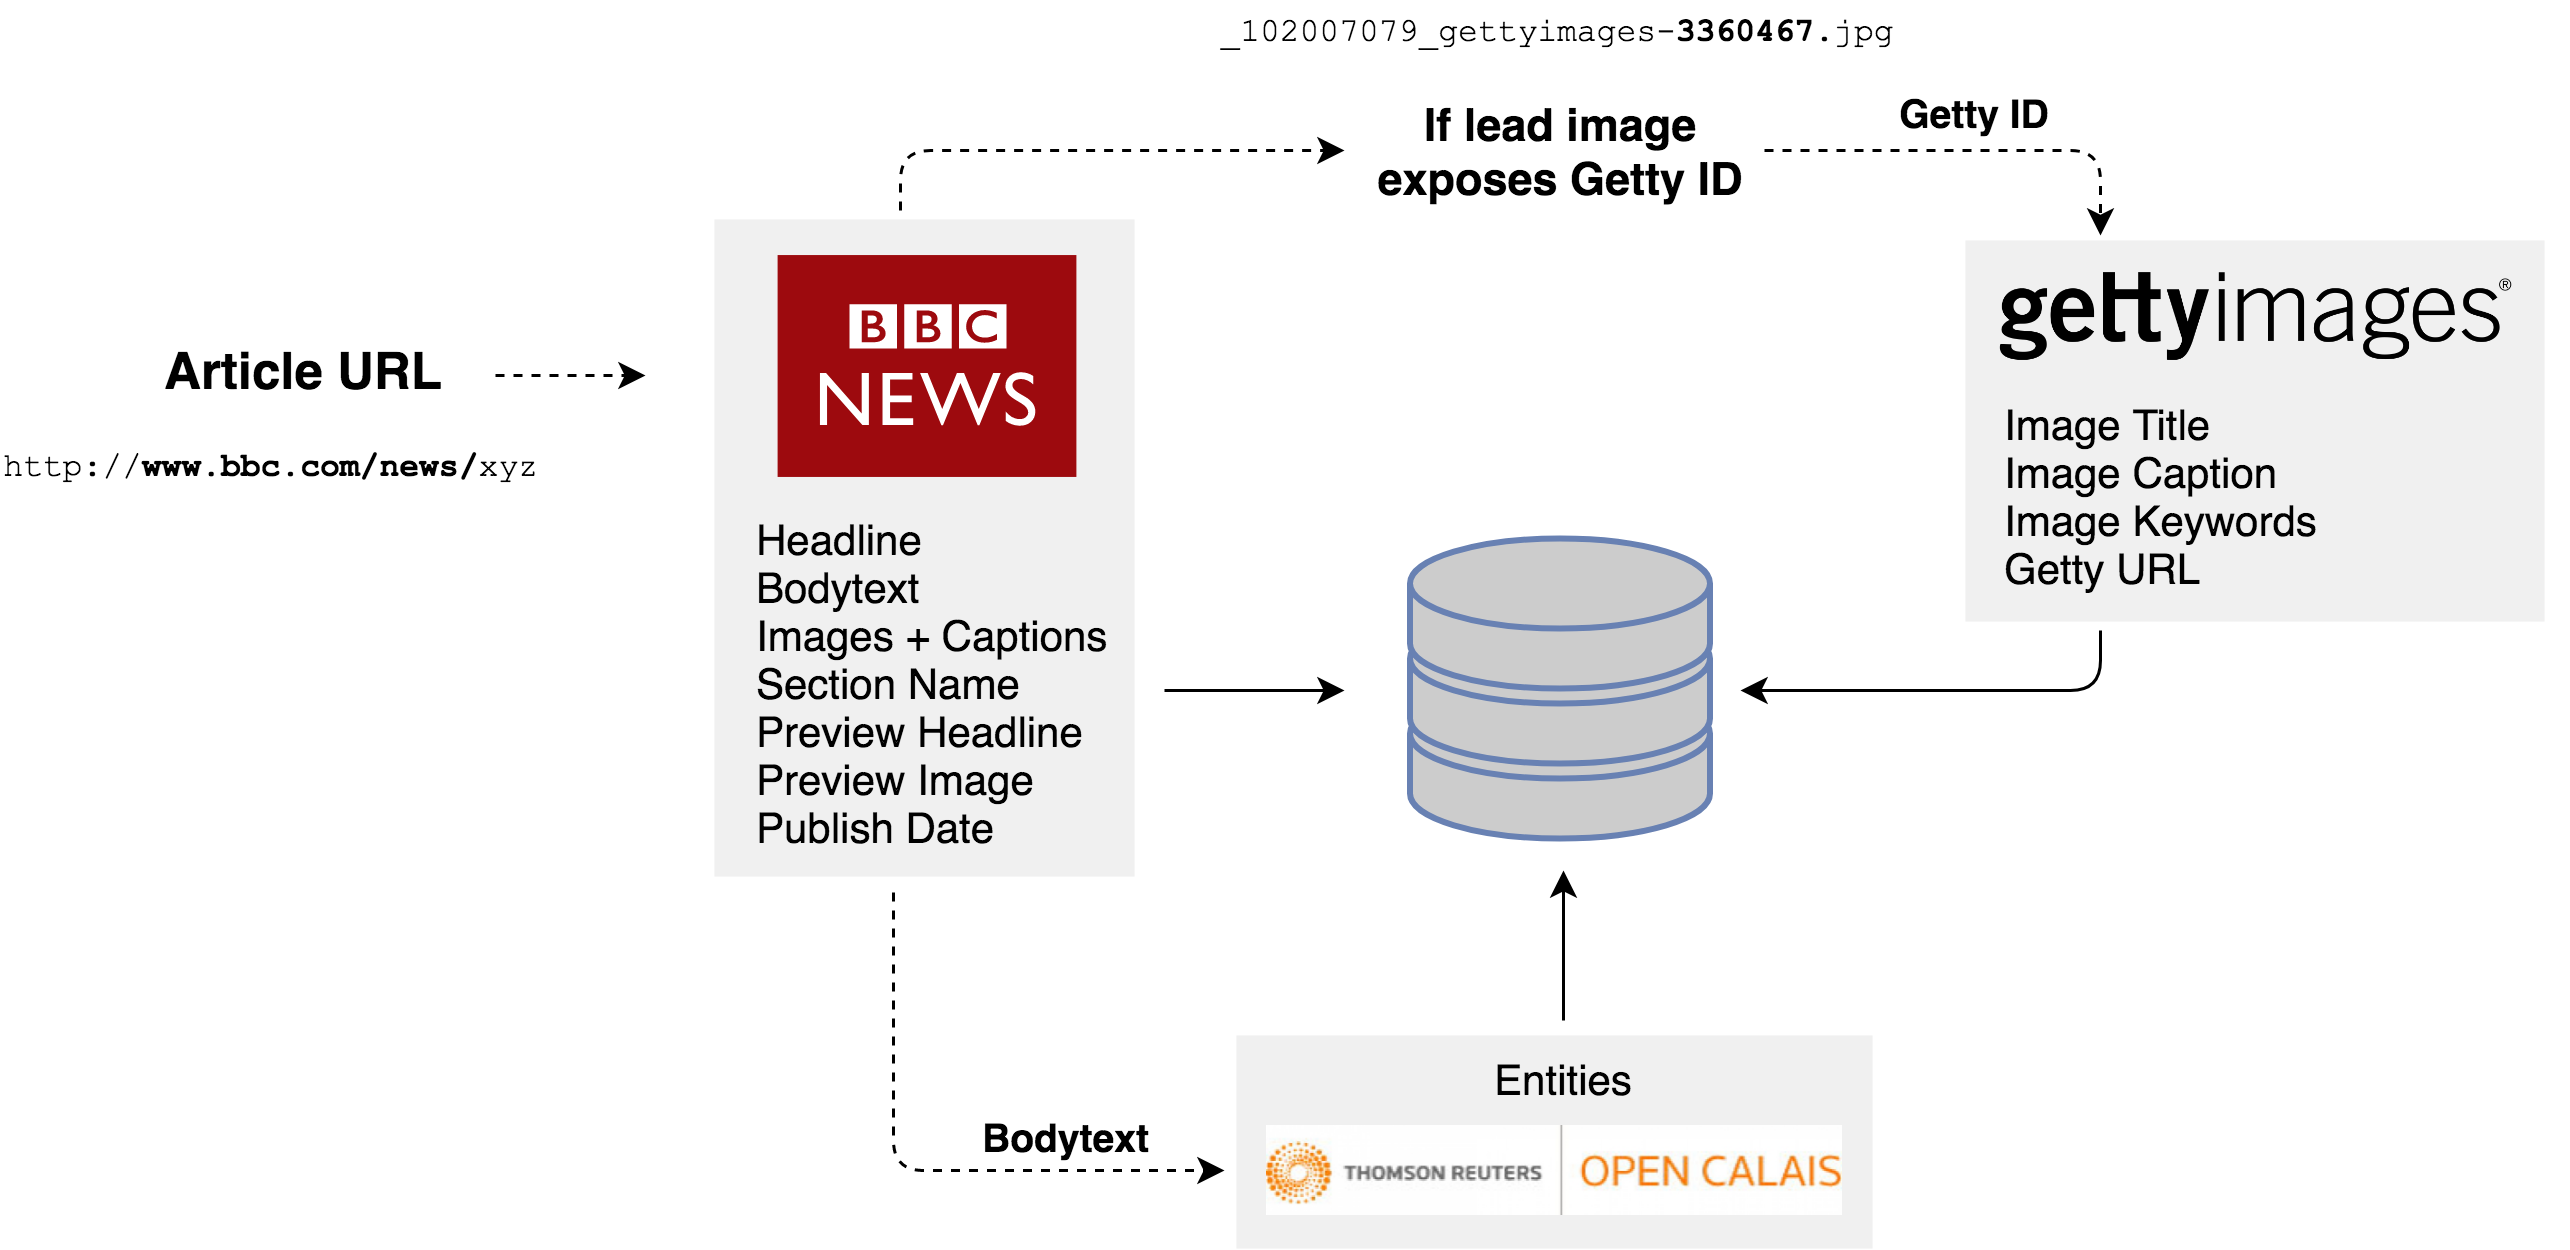
\includegraphics[width=\columnwidth]{picpic-scraper.png}
  \caption{Outline of the scraping procedure for one single article}
  \label{fig:picpic-scraper}
\end{figure}

Lorem ipsum dolor sit amet, consetetur sadipscing elitr, sed diam nonumy eirmod tempor invidunt ut labore et dolore magna aliquyam erat, sed diam voluptua. At vero eos et accusam et justo duo dolores et ea rebum. Stet clita kasd gubergren, no sea takimata sanctus est Lorem ipsum dolor sit amet. Lorem ipsum dolor sit amet, consetetur sadipscing elitr, sed diam nonumy eirmod tempor invidunt ut labore et dolore magna aliquyam erat, sed diam voluptua. At vero eos et accusam et justo duo dolores et ea rebum. Stet clita kasd gubergren, no sea takimata sanctus est Lorem ipsum dolor sit amet.

Lorem ipsum dolor sit amet, consetetur sadipscing elitr, sed diam nonumy eirmod tempor invidunt ut labore et dolore magna aliquyam erat, sed diam voluptua. At vero eos et accusam et justo duo dolores et ea rebum. Stet clita kasd gubergren, no sea takimata sanctus est Lorem ipsum dolor sit amet. Lorem ipsum dolor sit amet, consetetur sadipscing elitr, sed diam nonumy eirmod tempor invidunt ut labore et dolore magna aliquyam erat, sed diam voluptua. At vero eos et accusam et justo duo dolores et ea rebum. Stet clita kasd gubergren, no sea takimata sanctus est Lorem ipsum dolor sit amet.

\subsection{Preprocessing an Article} \label{SystemPreprocess}
\subsubsection{Features of a Term} \label{SystemPreprocessFeatures}
\subsubsection{Enhancing Preprocessing with Semantic Tagging} \label{SystemPreprocessCalais}

\subsection{Training Neural Networks} \label{SystemTrain}

\begin{figure}[t]
  %% Datei auf ganze Breite des Texts vergrößert
  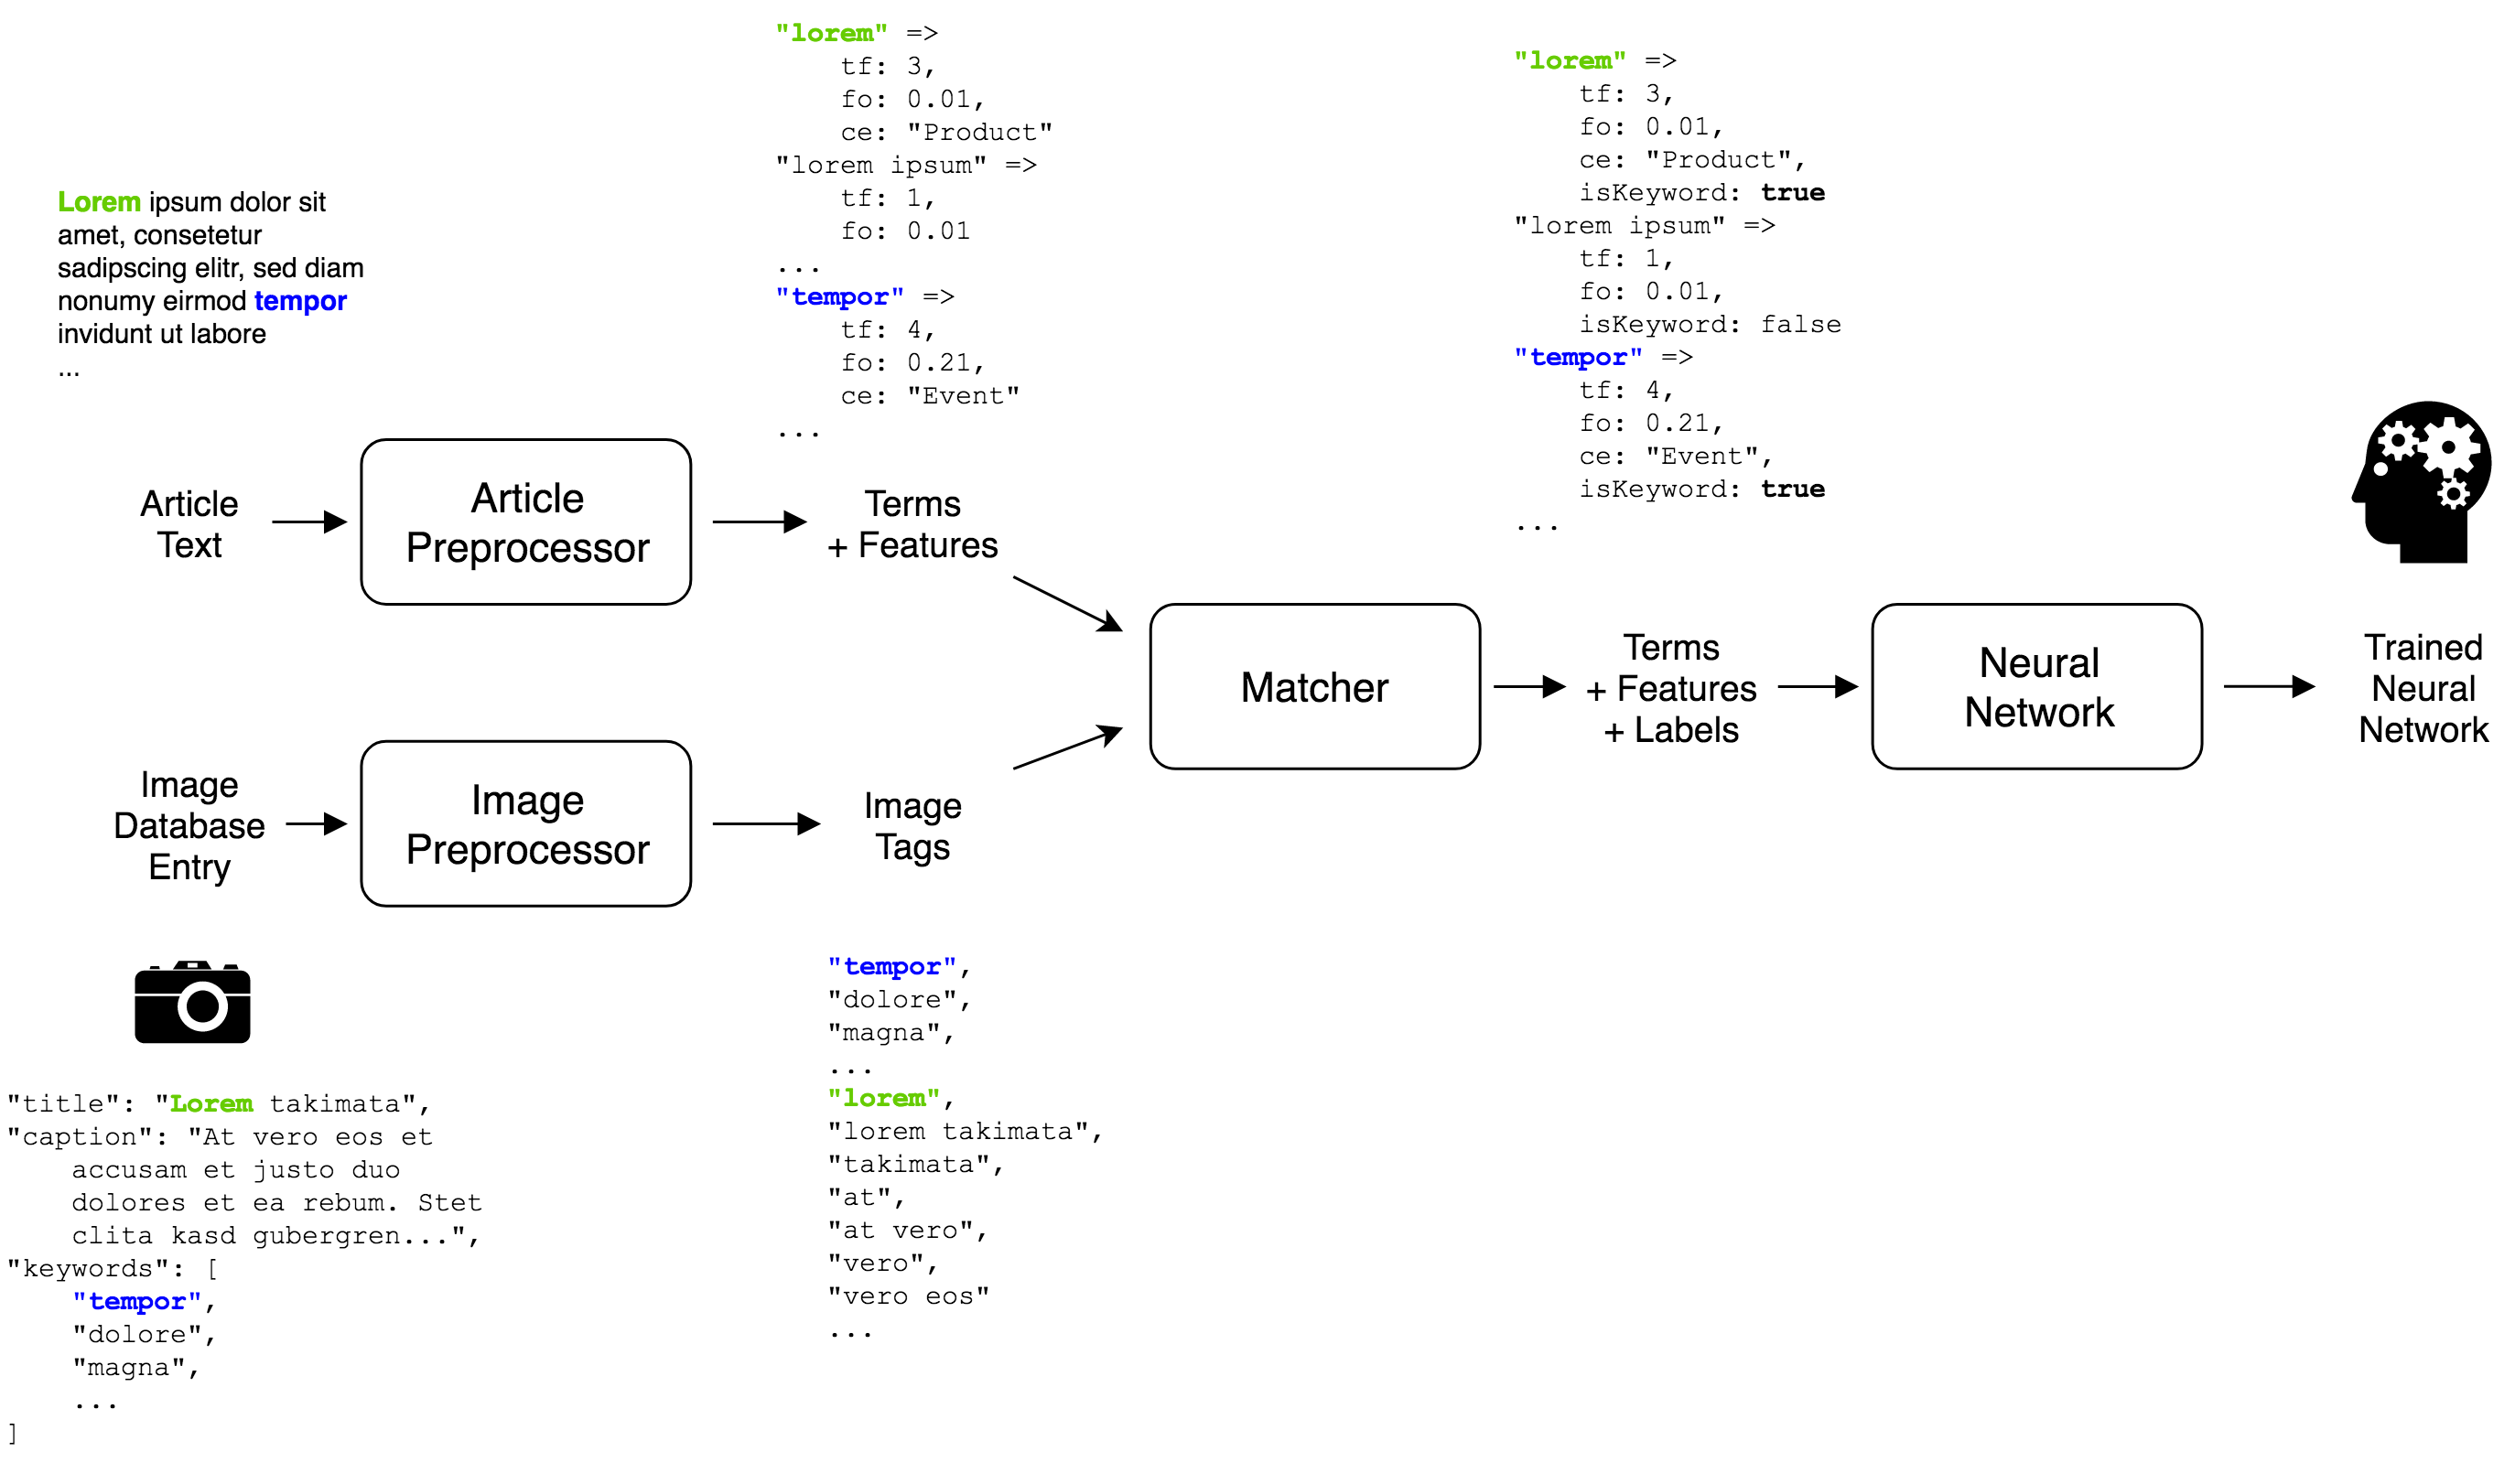
\includegraphics[width=\columnwidth]{picpic-training.png}
  \caption{Outline of the training pipeline}
  \label{fig:picpic-training}
\end{figure}

\subsubsection{Preprocessing an Image for Training} \label{SystemTrainPreprocess}
\subsubsection{Generating Training Data} \label{SystemTrainGenerate}
\subsubsection{Training the Networks} \label{SystemTrainTrain}

\subsection{Term Classification} \label{SystemClassification}
\subsubsection{Statistics Based Approach} \label{SystemClassificationStat}
\subsubsection{Machine Learning Based Approach} \label{SystemClassificationML}

\subsection{Image Query} \label{SystemQuery}

%______________________________________________________________________

\cleardoublepage

\section{Evaluation} \label{Eval}

\subsection{Factual Correctness as a Measure for System Performance} \label{EvalFacts}

\subsection{Evaluation Design} \label{EvalDesign}

\subsection{Evaluation Results} \label{EvalResults}

%______________________________________________________________________

\cleardoublepage

\section{Limitations}

\subsection{System Limitations}

\subsection{Research Design Limitations}

%______________________________________________________________________

\cleardoublepage

\section{Conclusion}

%______________________________________________________________________

% Der Befehl \cleardoublepage erscheint nur vor \section, nicht vor
% den "kleineren" Gliederungsbefehlen wie \subsection!
\cleardoublepage % Neue rechte Seite anfangen
\section{Example Section}

\begin{figure}%[btph]
  %% Datei ``beispielbild.eps'' oder ``beispielbild.png'', zentriert
  %\begin{center}\includegraphics{beispielbild}\end{center}

  %% Datei auf 8cm Breite verkleinert/vergrößert
  %\includegraphics[width=8cm]{beispielbild}
  %% Datei auf ganze Breite des Texts vergrößert
  %\includegraphics[width=\columnwidth]{beispielbild}
  %% Datei auf 60% der Textbreite verkleinert/vergrößert
  %\includegraphics[width=.6\columnwidth]{beispielbild}
  %% Weitere Optionen (Ausschnitt, drehen etc.) in der Doku zum graphicx-Paket

  \begin{center}\LARGE [BILD]\end{center}
  \caption{Bildunterschrift}
  \label{fig:beispielbild}
\end{figure}


Siehe Abbildung \ref{fig:beispielbild} oder einschlägige Literatur, z.B.
\cite[Seite 6]{Brill1992ATagger} oder \cite{Porter1980AnStripping}.

\bigskip % Größerer Abstand zum vorherigen Absatz
\textbf{Hinweis:} Die Verweise im generierten PDF (HTTP-Links, Verweise auf Kapitel oder Bilder) sind leicht eingefärbt. Wer das nicht will, z.B. weil es die Druckkosten erhöht, kann am Anfang des Dokuments \texttt{linkcolor} usw. auf ``black'' setzen.


\subsection{Medien}

\begin{figure}
  \begin{center}\LARGE [BILD]\end{center}
  \caption{Noch ein Bild}
  \label{fig:beispielbild2}
\end{figure}

\begin{itemize}
  \item Gesellschaftliche Medien
  \item Technische Medien
\end{itemize}


\subsection{Informatik}


\subsection{Medieninformatik}

\begin{description}
  \item[Medienwirkung:] Ein Spezialfach der Kommunikationswissenschaft. Für das erfolgreiche Studium des Anwendungsfachs Mediengestaltung ist eine künstlerische Begabung erforderlich.
  \item[Medienwirtschaft:] Ein Spezialfach der Betriebswirtschaftslehre
  \item[Mediengestaltung:] Ein Spezialfach der Kunstwissenschaft
\end{description}

\subsubsection{Was Sie schon immer wissen wollten, aber nie zu fragen
  wagten}

\paragraph{Überschrift}
Diese Überschrift erscheint fettgedruckt am Anfang des Absatzes.

\subsubsection{Was Sie nicht wissen wollten}

Text text textextext\footnote{Oder so ähnlich}.

%\_____________________________________________________________________

\cleardoublepage
\fancyhead[LE,RO,LO,RE]{} % Keine Kopfzeile mehr oben auf jeder Seite
\section*{Contents of the Attached CD}
%______________________________________________________________________

\cleardoublepage
%\begin{thebibliography}{99}

%\bibitem{Ivory01}

%  M.\ Y.\ Ivory, M.\ Hearts:
%  \href{http://www.ischool.washington.edu/myivory/thesis/thesis.pdf}{%
%    An Empirical Foundation for Automated Web Interface Evaluation}.
%  Ph.D. thesis, University of California at Berkeley, 2001


%\cleardoublepage
%\hspace{-\leftmargin}{\Large\bfseries Web-Referenzen} % Wüster Hack %-|

%\bibitem{NielsenAlertbox}

%  J.\ Nielsen: Alertbox: Current Issues in Web Usability
%  \url{http://useit.com/alertbox/}, accessed April~24, 2005.

%\end{thebibliography}

\bibliographystyle{plain}
\bibliography{mendeley_v2}

\end{document}
